\subsection{Labels and Referencing}
% \begin{frame}[c,plain,noframenumbering]
% \begin{tikzpicture}[remember picture,overlay]
% \fill[fill=gray]
%     (current page.south east)  rectangle ([shift={(0,-0.1\paperheight)}]current page.north west)   ;
% \end{tikzpicture}
% \centering
% \vfill
% \textcolor{white}{\Large\textbf{Referencing figures, tables,
% \\equations, algorithms, and listings}}
% \end{frame}

\begin{frame}[fragile]{Labels and Referencing}
    \noindent
    \Emph{A figure, table, equation, algorithm, listing has no place in a document, unless it is referenced!}

    \begin{columns}[t]
		\begin{column}{.5\textwidth}
            \begin{itemize}
                \item[]  \comm{label}{\textless label\textgreater} inside the environment to be referenced, and
                \item[] \comm{ref}{\textless label\textgreater} in the text.
            \end{itemize}     
            e.g., 
            \begin{itemize}
                \item[] \comm{caption}{Some fig. caption}\comm{label}{fig:cool-fig}.
                \item[] Fig.\texttildelow \comm{ref}{fig:cool-fig} becomes \texttt{Fig.~1}.
            \end{itemize}
		\end{column}
		\begin{column}{.5\textwidth}
			Use \pack{cleveref} and use correct naming conventions:
            \begin{description}
                \item[ch:] chapter
                \item[sec:] (sub)section 
                \item[fig:] figure
                \item[tab:] table
                \item[lst:] code listing
                \item[alg:] algorithm
                \item[app:] appendix (sub)section
            \end{description}
            \begin{itemize}
                \item[] \comm{cref}{fig:cool-fig} becomes \texttt{Fig.~1}.
            \end{itemize}
		\end{column}
    \end{columns}
\end{frame}

\begin{frame}[fragile]{Labels and Referencing}
%\vspace{.5cm}
	\begin{columns}[t]
		\begin{column}{.5\textwidth}
			\begin{figure}
			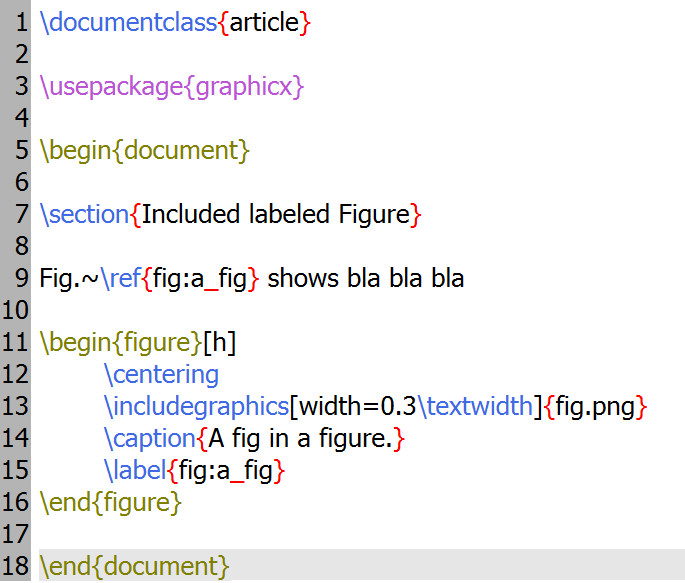
\includegraphics[scale=.5]{Figures/code7}
			\end{figure}
		\end{column}
		\begin{column}{.5\textwidth}
			\begin{figure}
			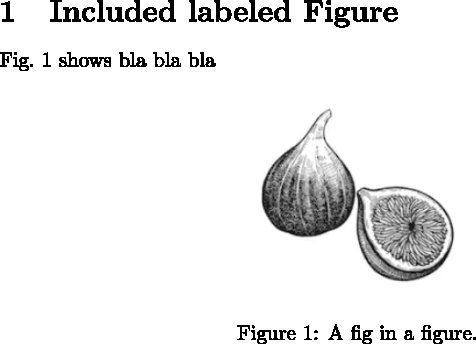
\includegraphics[width=.8\linewidth, frame, trim={-1cm -1cm -1cm -1cm},clip]{Figures/doc9}
			\end{figure}
		\end{column}
	\end{columns}
\end{frame}

\subsection{Bibliography}
% \begin{frame}[c,plain,noframenumbering]
% \begin{tikzpicture}[remember picture,overlay]
% \fill[fill=kul-blue]
%     (current page.south east)  rectangle  ([shift={(0,-0.1\paperheight)}]current page.north west)   ;
% \end{tikzpicture}
% \centering
% \vfill
% \textcolor{white}{\Large\textbf{Bibliography}}
% \end{frame}

\begin{frame}[fragile]{Bibliography}
Best practice
\vspace{.5cm}
	\\Resource you want to cite, must be provided to LaTeX in BibTex format
	\vskip.05\textheight
	Although you could store your BibTex directly in your .tex document,
	much better to store it in a separate .bib file, and point LaTeX to this file.
\end{frame}

\begin{frame}[fragile]{Bibliography}

In the preamble:
    \begin{itemize}
        \item[] \packopt{biblatex}{style=ieee}
        \item[] \commopt{addbibresource}{bib.bib}
        \item[] \commopt{AtBeginBibliography}{\textbackslash footnotesize}
    \end{itemize}
The last command is optional.
\somespace
Just before the end of the document:
    \begin{itemize}
        \item[] \commo{printbibliography}
    \end{itemize}
\end{frame}


\begin{frame}{natbib vs. biblatex}
    \textcolor{red}{TODO}
\end{frame}


\begin{frame}[containsverbatim, fragile]{BibTeX}
    \begin{minted}{latex}
    @ARTICLE{10460235,
      author={Callebaut, Gilles and Liu, Liang and 
      Eriksson, Thomas and Van der Perre, Liesbet and 
      Edfors, Ove and Fager, Christian},
      journal={IEEE Microwave Magazine}, 
      title={6G Radio Testbeds: Requirements, Trends, and Approaches}, 
      year={2024},
      volume={25},
      number={4},
      pages={14-31},
      doi={10.1109/MMM.2024.3351970}
    }
    \end{minted}
\end{frame}


\begin{frame}[fragile]{Bibliography}
On IEEEXplore
%\vspace{.5cm}
	\begin{figure}
		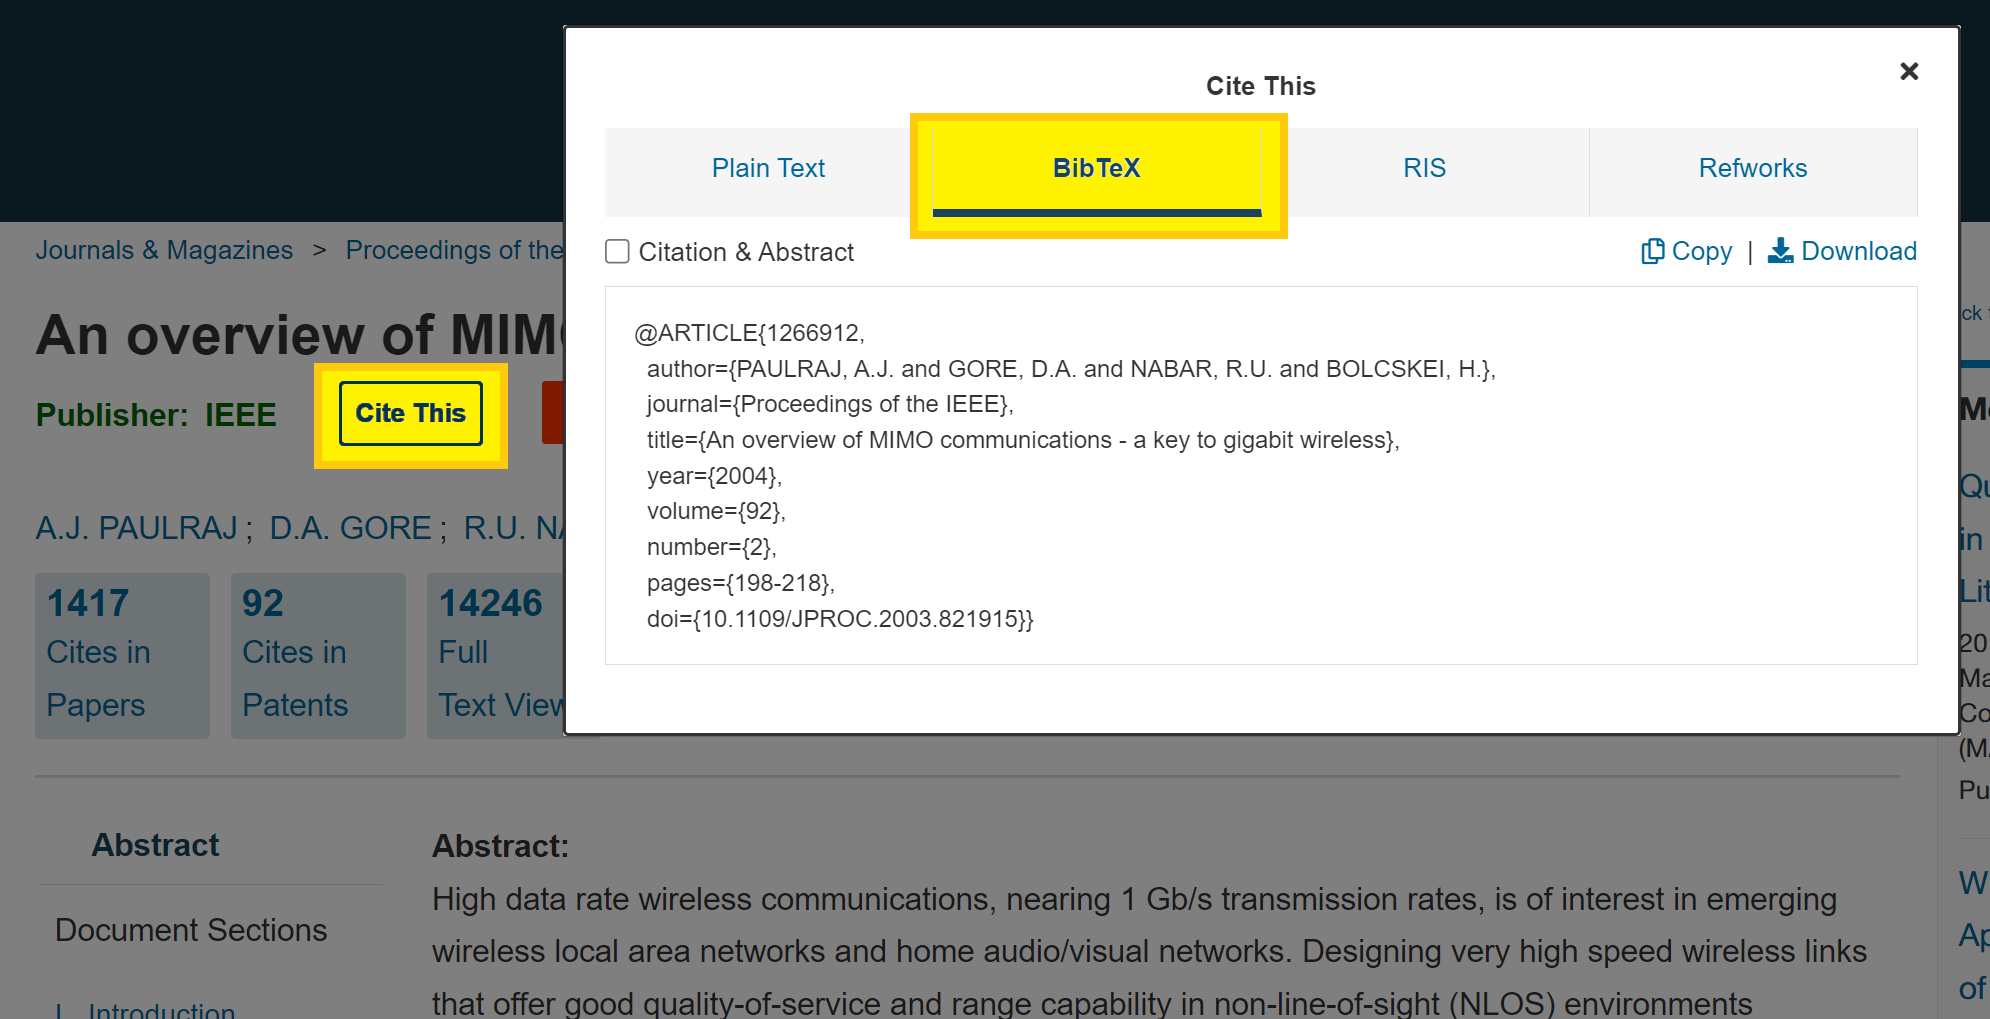
\includegraphics[width=.7\linewidth]{Figures/bib_1}
	\end{figure}
\end{frame}

\begin{frame}[fragile]{Bibliography}
    \begin{columns}[t]
		\begin{column}{.5\textwidth}
			Citing a reference
        \somespace
	Optional, but to prettify citations \\\pack{cite}  \Emph{($\leftarrow$ only if you are not using biblatex)}
	\somespace
	In text: 
	\\``\texttt{\ldots using a reference\textcolor{orange}{$\mathbf\sim$}\comm{cite}{citekey}}''
	\somespace
	$\sim$ is a fixed space. This prevents a line-break on this space. 
    \somespace
    \Emph{Always insert $\sim$ before \comm{cite}{}.}
		\end{column}
		\begin{column}{.5\textwidth}
			\begin{figure}
			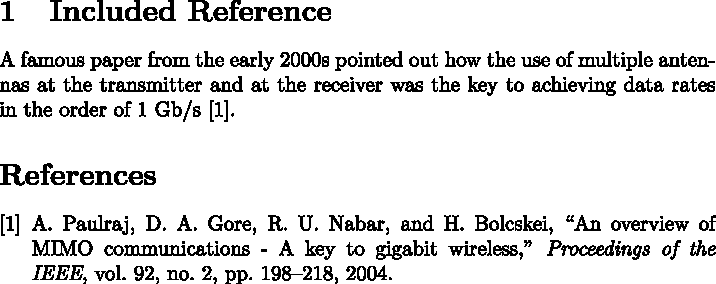
\includegraphics[width=.9\linewidth, frame, trim={-1cm -1cm -1cm -1cm},clip]{Figures/doc10}
			\end{figure}
		\end{column}
	\end{columns}
\end{frame}

\begin{frame}[fragile]{Bibliography}
\vspace{.5cm}
	\begin{figure}
		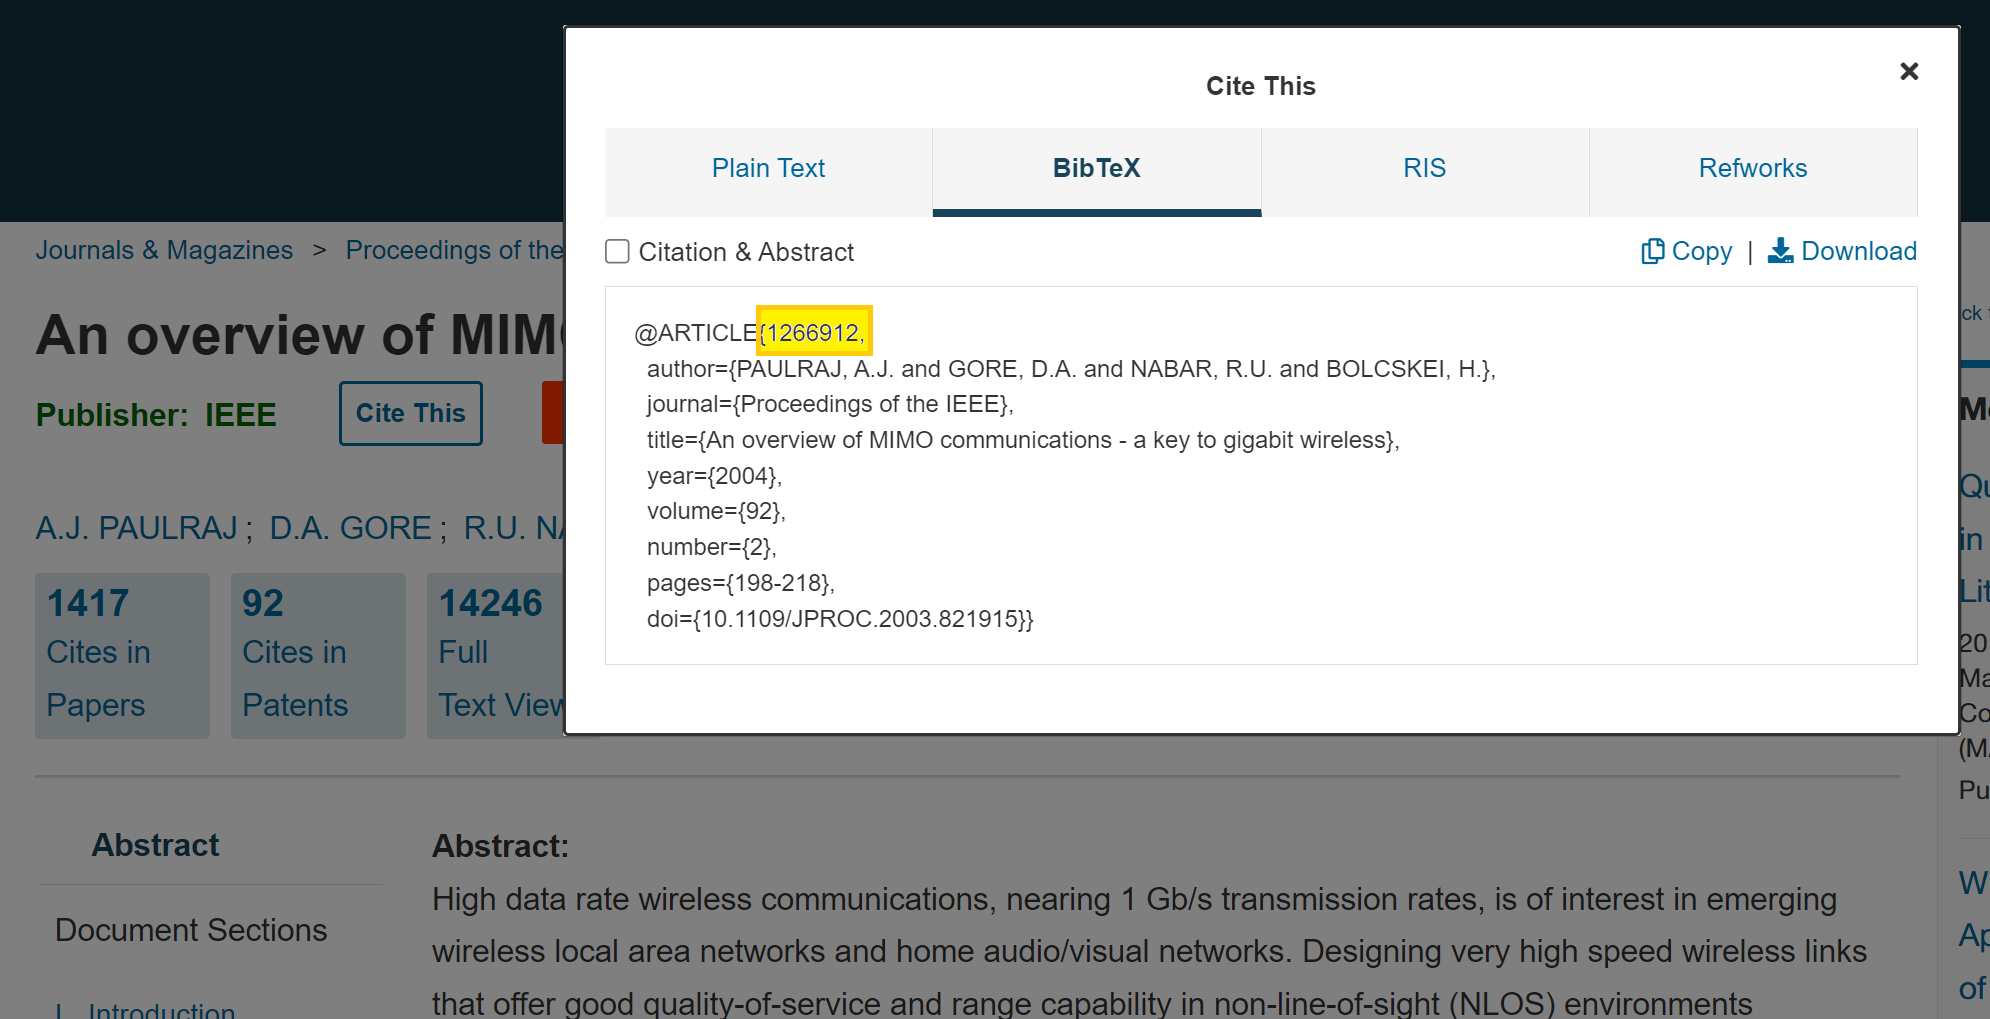
\includegraphics[width=.7\linewidth]{Figures/bib_2}
	\end{figure}
\end{frame}

\begin{frame}[fragile]{Cleaning BibTeX file}
\centering
	\begin{figure}
		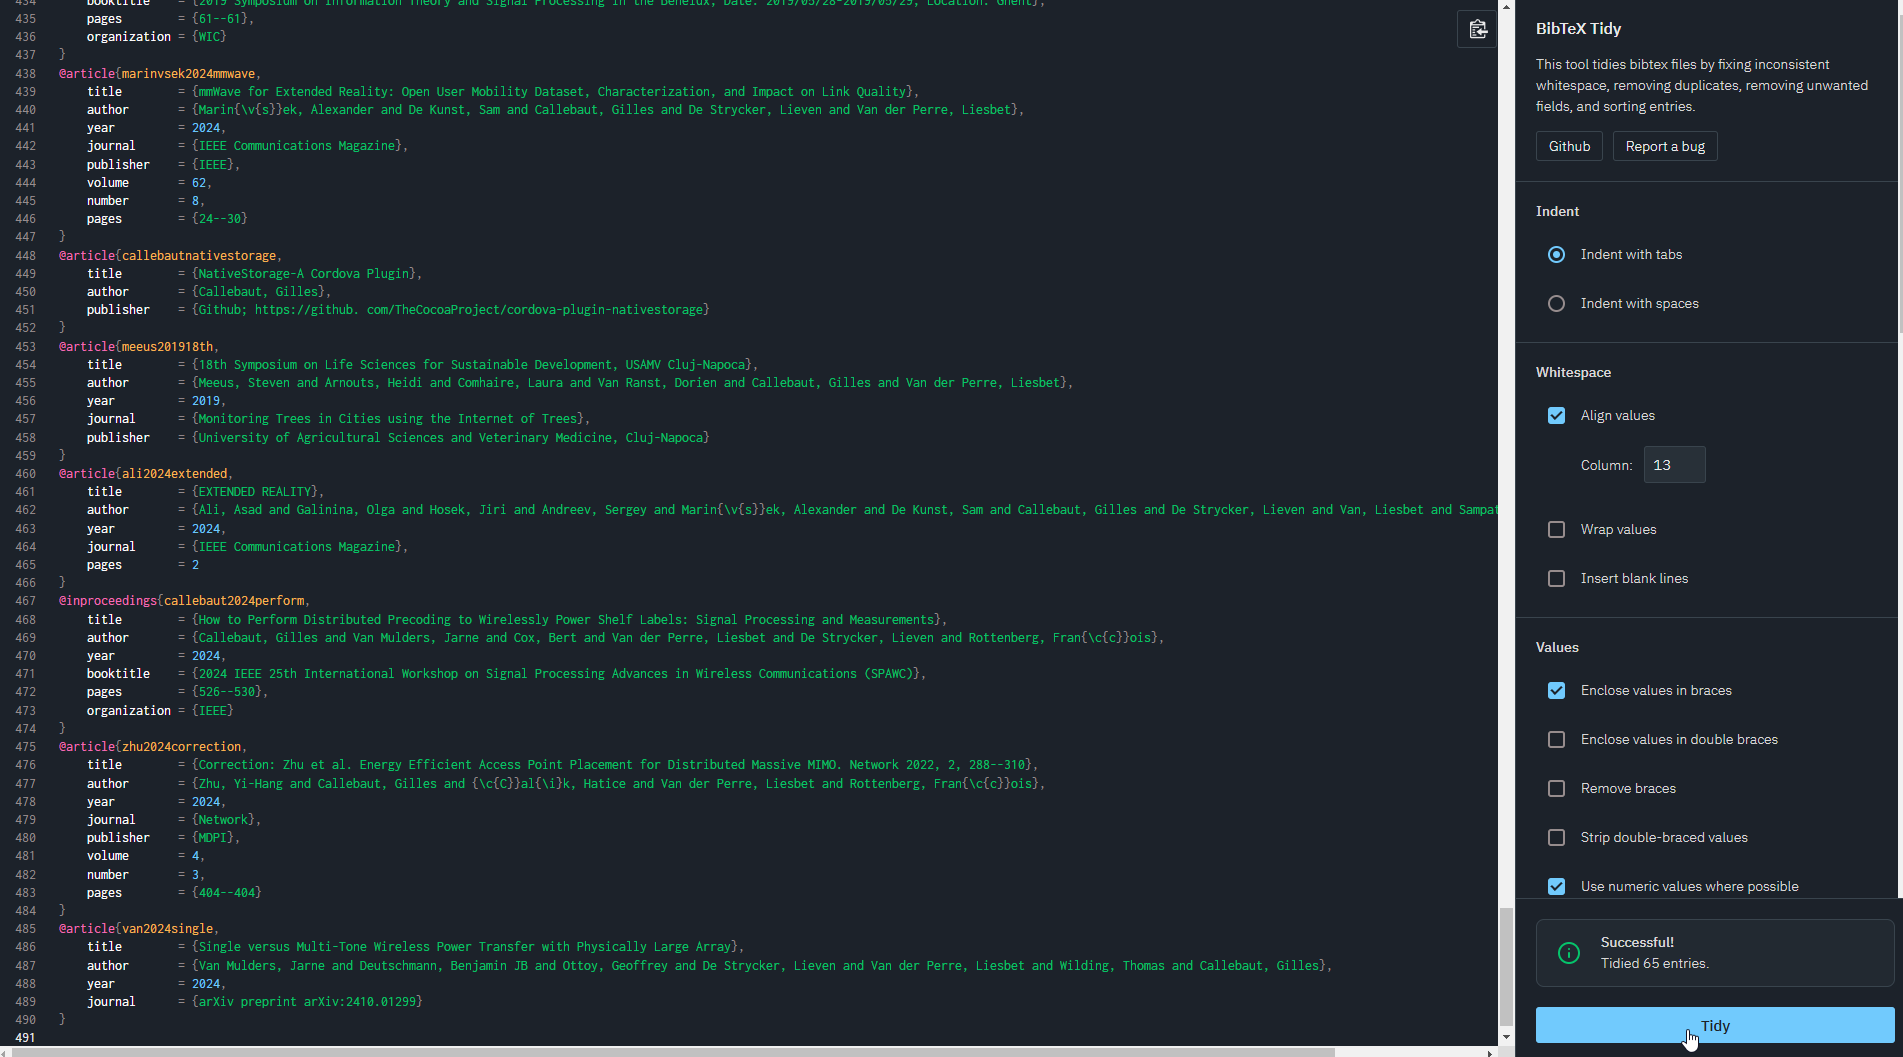
\includegraphics[width=.7\linewidth]{Figures/bib3.png}
	\end{figure}
    \url{https://flamingtempura.github.io/bibtex-tidy}
\end{frame}

% \begin{frame}[fragile]{Bibliography}
% %\vspace{.5cm}
% 	\begin{columns}[t]
% 		\begin{column}{.5\textwidth}
% 			\begin{figure}
% 			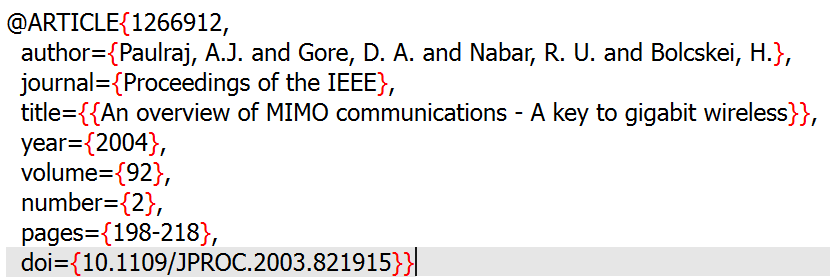
\includegraphics[scale=.4]{Figures/code8_1}{\tiny \quad refs.bib file}
% 			\vskip.03\textheight
% 			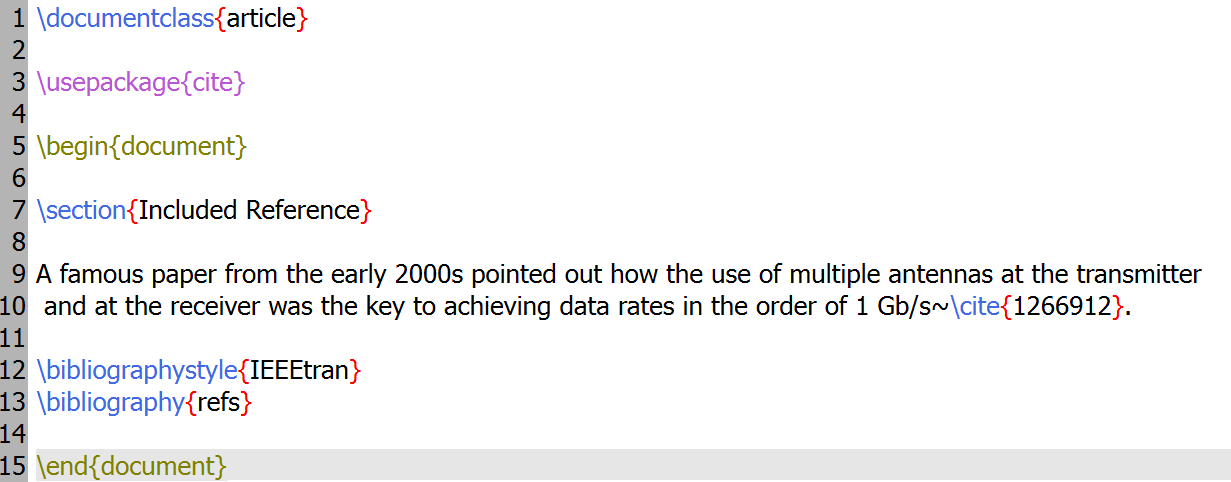
\includegraphics[scale=.4]{Figures/code8_2}
% 			\end{figure}
% 		\end{column}
% 		\begin{column}{.5\textwidth}
% 			\begin{figure}
% 			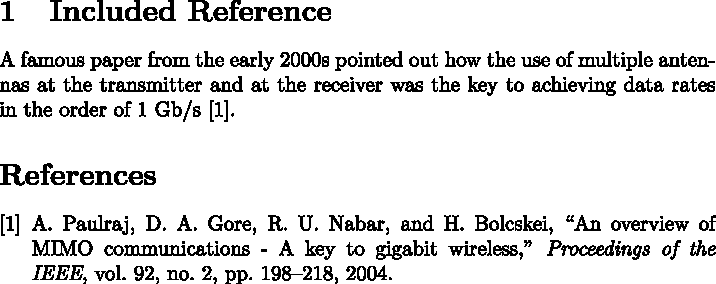
\includegraphics[width=.9\linewidth, frame, trim={-1cm -1cm -1cm -1cm},clip]{Figures/doc10}
% 			\end{figure}
% 		\end{column}
% 	\end{columns}
% \end{frame}


\begin{frame}[fragile]{Want to know more about Ref.~Managers and BibTeX?}
Or more general information about information retrieval?
\vspace{.5cm}
	\\Contact colleague Eef Soete (\href{mailto:eef.soete@kuleuven.be}{eef.soete@kuleuven.be})
	\somespace
	\begin{figure}
		
\includegraphics[width=.5\linewidth]{Figures/Eef_profile}
	\end{figure}
\end{frame}


% \begin{frame}[fragile,c]{Goal of today}
% Show you the basics
% \begin{itemize}
% 	\item Starting a document
% 	\item Text structuring
% 	\item Figures, Tables, Equations, Algorithms, and Listings
% 	\item Bibliography
% \end{itemize}	
% \vskip.05\textheight
% \textbf{What if you need more than the basics?}
% \vskip.05\textheight
% Try it yourself!
% \end{frame}

% \begin{frame}[fragile]{What if you need more than the basics?}
% \vspace{.5cm}
% \href{https://en.wikibooks.org/wiki/LaTeX}{https://en.wikibooks.org/wiki/LaTeX}
% \\\href{https://tex.stackexchange.com/}{https://tex.stackexchange.com/}
% \\\href{https://www.overleaf.com/learn}{https://www.overleaf.com/learn}
% \vskip.05\textheight
% \begin{figure}
% 	
\includegraphics[width=.25\linewidth]{Figures/google-is-your-friend}
% 	\hskip.05\textwidth
% 	
\includegraphics[width=.15\linewidth]{Figures/chatgpt}
% \end{figure}
% \end{frame}


% \begin{frame}[c]{}
% \tikzstyle{startstop} = [rectangle, minimum width=3cm, minimum height=1cm,text centered, draw=black, fill=red!30]
% \tikzstyle{process} = [rectangle, minimum width=3cm, minimum height=1cm, text centered, draw=black, fill=blue!30]
% \tikzstyle{data} = [rectangle, minimum width=3cm, minimum height=1cm, text centered, draw=black, fill=green!30]
% \tikzstyle{arrow} = [thick,->,>=stealth]

% \resizebox{!}{0.8\textheight}{%
% \begin{tikzpicture}[node distance=2cm]

% % Nodes
% \node (source) [process] {Source};
% \node (biblatex) [data, right=3cm of source] {biblatex};
% \node (style) [process, right=3cm of biblatex] {Style};
% \node (bibdata) [process, below=1.5cm of style] {Bib data};
% \node (pdflatex1) [process, below=2cm of source] {pdflatex};
% \node (bibtex) [process, right=3cm of pdflatex1] {bibtex};
% \node (logfile1) [process, right=3cm of bibtex] {Log file};
% \node (pdflatex2) [process, below=2cm of pdflatex1] {pdflatex};
% \node (pdflatex3) [process, below=2cm of pdflatex2] {pdflatex};
% \node (logfile2) [process, right=3cm of pdflatex2] {Log file};
% \node (pdffile) [startstop, below=2cm of pdflatex3] {PDF file};

% % Arrows
% \draw [arrow] (source) -- (biblatex);
% \draw [arrow] (biblatex) -- (style);
% \draw [arrow] (biblatex) -- (bibdata);
% \draw [arrow] (source) -- (pdflatex1);
% \draw [arrow] (pdflatex1) -- (bibtex);
% \draw [arrow] (bibtex) -- (logfile1);
% \draw [arrow] (bibtex) |- (pdflatex2);
% \draw [arrow] (pdflatex2) -- (logfile2);
% \draw [arrow] (pdflatex2) -- (pdflatex3);
% \draw [arrow] (pdflatex3) -- (pdffile);

% \end{tikzpicture}}
% \end{frame}